\documentclass[11pt]{article}

\usepackage[margin=1in]{geometry}
\usepackage{amsmath,amssymb,amsfonts}
\usepackage{booktabs}
\usepackage{graphicx}
\usepackage{hyperref}
\usepackage{xcolor}
\usepackage{longtable}
\usepackage{pdflscape}
\usepackage{multirow}
\usepackage[affil-it]{authblk}
\usepackage{tikz}
\usetikzlibrary{arrows.meta, positioning}
\usepackage{lineno}
\usepackage{natbib}

\renewcommand{\arraystretch}{1.3}

\title{Abundance or Activity? Mechanism-Dependent Validity of \emph{Cis}-pQTL Mendelian Randomization}

\author{Elliot Tower}
\affil{Independent researcher \\ \texttt{elliot@elliottower.ai}}

\begin{document}
\linenumbers
\maketitle

\begin{abstract}
A \emph{cis}-pQTL instrument measures lifelong variation in circulating protein abundance, yet evaluations of pQTL-based Mendelian randomization (MR) for drug-target validation report composite accuracy across all drug mechanisms. This conflation predicts a mechanism-dependent domain of validity: MR should be informative when drug and instrument act on the same causal axis (protein level) and uninformative when they do not (protein function). We tested this prediction in a pre-registered, outcome-blind evaluation of a zero-parameter classifier ($p < 0.05 \rightarrow$ predict SUCCESS) against 195 Phase~III drug-target pairs across 24 diseases. For activity-blocking targets ($n = 76$), MR is uninformative (balanced accuracy [BA] $= 0.511$, 90\% CI $[0.456, 0.576]$), robust to every missingness scenario. For abundance-modulating targets ($n = 59$), MR trends positive (BA $= 0.590$, $[0.496, 0.691]$; AUC $= 0.595$, permutation $p = 0.038$). The pooled BA of $0.559$ is a mixture of these strata, consistent with benchmarks reporting lower pQTL enrichment than GWAS-only approaches. A pre-registered second instrument (pLoF burden, $n = 132$) returned null results, reflecting the power wall for rare-variant confirmation. The instrument class has a definable validity boundary set by drug mechanism. Six protocol versions, each SHA-256 hashed before execution, ensure full outcome-blindness.
\end{abstract}

\noindent\textbf{Keywords:} Mendelian randomization, \emph{cis}-pQTL, drug-target validation, instrument validity, protein quantitative trait locus, mechanism of action, pre-registration

\section{Introduction}
\label{sec:intro}

Mendelian randomization (MR) using a \emph{cis}-acting protein quantitative trait locus (pQTL) estimates the causal effect of lifelong variation in circulating protein abundance on disease risk \cite{gill2021mendelian}. A \emph{cis}-pQTL---a genetic variant near a gene that changes how much of that gene's protein circulates in blood---serves as a natural randomization of protein exposure, conceptually mimicking a randomized trial of a drug that perturbs the same target. This logic has motivated the use of pQTL-MR as a drug-target validation tool, building on the observation that targets with genetic support have approximately twice the historical Phase~III approval rate \cite{nelson2015support, king2019greater, minikel2024refining}.

Yet this ${\sim}2\times$ genetic lift treats all drug mechanisms as interchangeable. The instrument measures one specific quantity: circulating protein \emph{level}. Drugs that modulate protein abundance---biologics that deplete a circulating target, antisense oligonucleotides that reduce translation---act on this same causal axis, so the MR estimate is relevant to the drug's mechanism. Drugs that block enzymatic \emph{activity} or antagonize a receptor without changing the target protein's measured level act on a different axis entirely. For these activity-blocking drugs, a pQTL-based MR estimate answers ``what happens with less of this protein?'' when the drug asks ``what happens when this protein's function is blocked?'' Gill et al.\ (\citeyear{gill2021mendelian}) noted this distinction conceptually; we provide the first empirical test of whether it predicts a measurable validity boundary.

This axis mismatch predicts a \emph{mechanism-dependent domain of validity}: pQTL-MR should be informative where instrument and drug share a causal axis and uninformative where they do not. Recent composite pQTL benchmarks support this prediction indirectly. Rao et al.\ (\citeyear{rao2023pqtl}) found that pQTL-GWAS enrichment for approved targets (OR $= 1.31$) underperforms GWAS-only enrichment (OR $= 2.17$), consistent with a pooled pQTL signal being diluted by mechanism-inappropriate targets.

\begin{figure}[t]
\centering
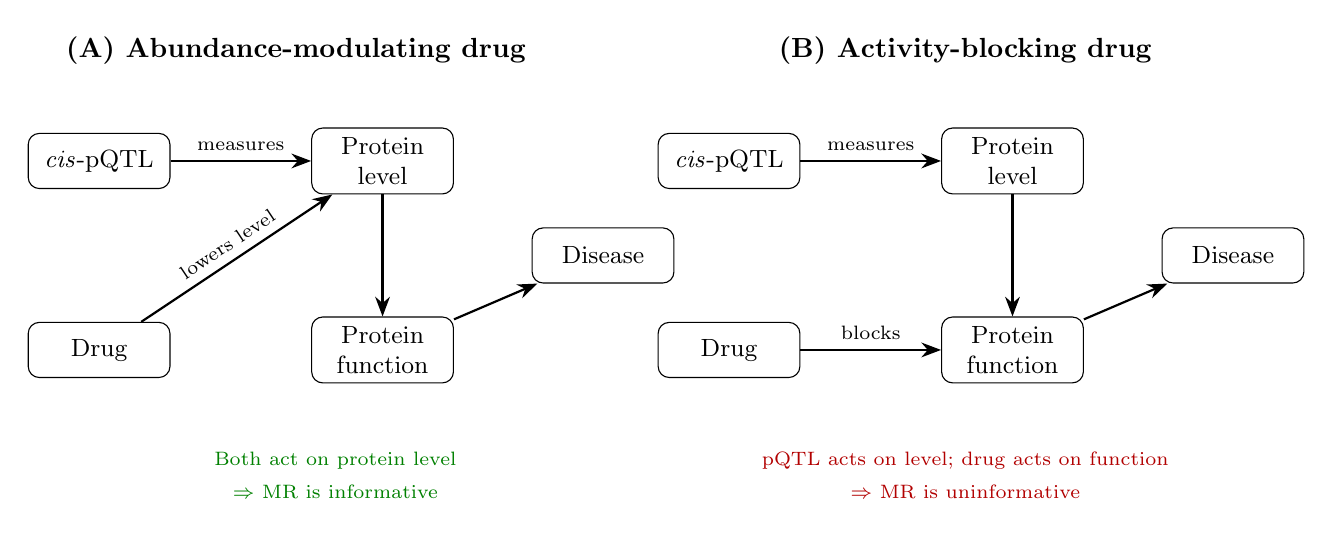
\begin{tikzpicture}[
    every node/.style={font=\small},
    box/.style={draw, rounded corners, minimum width=1.8cm, minimum height=0.7cm, align=center},
    arr/.style={-{Stealth[length=2.5mm]}, thick},
]

\node[font=\normalsize\bfseries] at (2.5, 1.4) {(A) Abundance-modulating drug};

\node[box] (snpA) at (0, 0) {\emph{cis}-pQTL};
\node[box] (lvlA) at (3.6, 0) {Protein\\level};
\node[box] (funA) at (3.6, -2.4) {Protein\\function};
\node[box] (disA) at (6.4, -1.2) {Disease};
\node[box] (drugA) at (0, -2.4) {Drug};

\draw[arr] (snpA) -- node[above, font=\scriptsize, midway] {measures} (lvlA);
\draw[arr] (lvlA) -- (funA);
\draw[arr] (funA) -- (disA);
\draw[arr] (drugA) -- node[above, font=\scriptsize, midway, sloped] {lowers level} (lvlA);

\node[font=\scriptsize, green!50!black] at (3, -3.8) {Both act on protein level};
\node[font=\scriptsize, green!50!black] at (3, -4.2) {$\Rightarrow$ MR is informative};

\begin{scope}[xshift=8cm]

\node[font=\normalsize\bfseries] at (3, 1.4) {(B) Activity-blocking drug};

\node[box] (snpB) at (0, 0) {\emph{cis}-pQTL};
\node[box] (lvlB) at (3.6, 0) {Protein\\level};
\node[box] (funB) at (3.6, -2.4) {Protein\\function};
\node[box] (disB) at (6.4, -1.2) {Disease};
\node[box] (drugB) at (0, -2.4) {Drug};

\draw[arr] (snpB) -- node[above, font=\scriptsize, midway] {measures} (lvlB);
\draw[arr] (lvlB) -- (funB);
\draw[arr] (funB) -- (disB);
\draw[arr] (drugB) -- node[above, font=\scriptsize, midway, sloped] {blocks} (funB);

\node[font=\scriptsize, red!70!black] at (3, -3.8) {pQTL acts on level; drug acts on function};
\node[font=\scriptsize, red!70!black] at (3, -4.2) {$\Rightarrow$ MR is uninformative};

\end{scope}

\end{tikzpicture}
\caption{Causal structure of \emph{cis}-pQTL Mendelian randomization under two drug mechanisms. Both panels share the same causal chain: protein level determines protein function, which determines disease risk. (A)~An abundance-modulating drug reduces protein level---the same node the genetic instrument acts on---so MR estimates the drug-relevant effect. (B)~An activity-blocking drug blocks protein function directly (the protein is still present at normal levels but cannot act). The genetic instrument still measures protein level, so MR answers ``what happens with less protein?'' when the drug asks ``what happens when the protein is blocked?''---a structural mismatch independent of sample size.}
\label{fig:dag}
\end{figure}

We test this prediction in a pre-registered, outcome-blind evaluation of a frozen, zero-parameter MR classifier against 195 Phase~III drug-target pairs across 24 diseases. The evaluation has three properties that distinguish it from prior retrospective analyses. First, the evaluable set is the mechanical intersection of an independent pQTL catalog and an independent drug database, neither of which references clinical outcomes, eliminating the possibility of tuning inclusion criteria to the answer. Second, the classifier ($p < 0.05 \rightarrow$ predict SUCCESS) carries zero free parameters, removing degrees of freedom that retrospective analyses retain. Third, the protocol evolved across six publicly versioned iterations (V1--V3.4), each SHA-256 hashed before execution with a documented deviation log.

\section{Methods}
\label{sec:methods}

\paragraph{Data sources.}
Genetic instruments were drawn from two sources: the published EpiGraphDB \emph{cis}-pQTL MR catalog \cite{zheng2020phenome}, based on the INTERVAL study (${\sim}1{,}740$ proteins, $N \approx 3{,}300$, SomaScan), and UK Biobank Pharma Proteomics Project (UKB-PPP) \emph{cis}-pQTLs (${\sim}2{,}900$ proteins, $N \approx 54{,}000$, Olink). Each protein used one instrument: the sentinel \emph{cis}-pQTL (lowest $p$ among conditionally independent \emph{cis} signals as reported by the source study; no additional conditional analysis was performed). Multi-SNP IVW \citep{burgess2013ivw} and \emph{trans}-pQTL results were excluded a priori because of their vulnerability to horizontal pleiotropy. When \emph{cis}-pQTLs existed in both sources, the source with the largest discovery $N$ for that protein was used; the MR $p$-value was never used to select instruments. Drug targets were taken from the Open Targets Platform \cite{ochoa2021opentargets}, from which all compounds reaching Phase~III were retrieved and linked to their mechanistic gene targets algorithmically.

\paragraph{Outcome GWAS.}
For each disease, a non-UKB outcome GWAS was selected to avoid sample overlap with UKB-PPP instruments. Sources included FinnGen R10, CARDIoGRAMplusC4D, IMSGC, PGC, IIBDGC, ILCCO/TRICL, and disease-specific consortia (full mapping in Supplementary~S1). Seven chronic kidney disease pairs used a UKB-derived outcome GWAS (no non-UKB alternative with adequate $N$) and were flagged for sensitivity analysis. Two diseases (juvenile idiopathic arthritis, neuroblastoma) had no GWAS available on OpenGWAS. MR estimates were single-SNP Wald ratios: $\hat{\beta} = \beta_{\text{outcome}} / \beta_{\text{exposure}}$, $\text{SE} = |\text{SE}_{\text{outcome}} / \beta_{\text{exposure}}|$. Instrument strength was not formally assessed via $F$-statistics because individual-level data were not available; however, \emph{cis}-pQTLs from UKB-PPP ($N \approx 54{,}000$) typically have $F > 100$, and even INTERVAL ($N \approx 3{,}300$) sentinels have $F > 20$ given the large effect sizes characteristic of protein-altering \emph{cis} variants. Winner's curse from discovery-sample inflation \citep{burgess2011weak} may attenuate MR estimates by $20$--$40\%$ for INTERVAL-derived instruments, biasing toward the null and inflating false negatives---a conservative direction.

\paragraph{Pre-registration protocol.}
The protocol evolved across six publicly versioned iterations (V1--V3.4), each SHA-256 hashed before execution, with all amendments timestamped and justified in the deviation log (Supplementary~S1). V3.4 expanded V3.3 ($n = 50$) by adding UKB-PPP instruments and broadening the disease universe, motivated solely by insufficient power at V3.3 (the V3.3 BA~CI included $0.50$). The candidate universe was frozen (SHA-256: \texttt{c428c733...}; full hash in the repository) before outcome adjudication. The expansion from V3.3 to V3.4 was planned before examining V3.3 outcomes by mechanism stratum and was motivated solely by insufficient statistical power (the V3.3 composite BA~CI included $0.50$).

\paragraph{Outcome adjudication.}
Outcome labels were adjudicated independently against FDA/EMA records and ClinicalTrials.gov. SUCCESS denotes regulatory approval or a met Phase~III primary endpoint; FAILURE denotes a failed primary endpoint or discontinuation. A TARGET\_MISMATCH exclusion rule removed pairs where the drug acts on a different protein than the pQTL target. To avoid asymmetric scrutiny, the mismatch audit was applied to all pairs.

\paragraph{Mechanism classification.}
Each pair was classified by drug mechanism of action into one of three strata: \emph{abundance-modulating} (the drug reduces circulating protein level or blocks a soluble ligand, matching the pQTL perturbation), \emph{activity-blocking} (the drug inhibits enzymatic activity or blocks a receptor without changing the target protein's measured circulating level), or \emph{mixed} (both mechanisms apply). Classification was determined by the drug's pharmacological action, not the MR result. The boundary is not always sharp: some receptor antagonists can indirectly perturb measured protein levels through feedback upregulation or receptor internalization. Tocilizumab (anti-IL6R) was classified as abundance-modulating because the \emph{cis}-pQTL instruments soluble IL-6 receptor level, and tocilizumab blocks a soluble ligand-receptor axis---the drug reduces IL-6 signaling by sequestering the soluble receptor, acting on the same molecular species the instrument measures. Other edge cases were classified by primary pharmacological mechanism. The mixed stratum ($n = 3$) was too small for standalone analysis and was pooled only. Mechanism classification was performed before outcome adjudication (as part of the V3.4 protocol freeze) and the full per-pair classification table is available in the repository for independent verification.

\paragraph{Classifier.}
The classifier carries zero free parameters: MR $p < 0.05 \rightarrow$ predict SUCCESS; MR $p \geq 0.05 \rightarrow$ predict FAILURE. The threshold $p < 0.05$ is the field-standard MR significance criterion and was not optimized on these data.

\paragraph{Statistical analysis.}
The co-primary metrics were (i)~pooled balanced accuracy with 10{,}000-iteration bootstrap 90\% CI (chosen over 95\% because the pre-registered falsification criterion required the CI lower bound to exceed $0.50$; a 90\% CI provides a more stringent test of this one-sided criterion) and (ii)~mechanism-stratified BA. AUC was computed using the Wilcoxon--Mann--Whitney $U$-statistic with $-\log_{10}(p)$ as the continuous score, and significance assessed by 10{,}000-label permutation. A pre-declared falsification criterion required the \emph{pooled} BA~CI lower bound to exceed $0.50$ (met: pooled 90\% CI lower bound $= 0.503$); this criterion was applied to the composite, not to individual strata. All hypotheses and analysis specifications were pre-declared before adjudication.

\section{Results}

\subsection{Candidate funnel}
\label{sec:funnel}

From 211 unique gene--disease pairs at the intersection of pQTL instruments and Open Targets Phase~III targets, 195 were evaluable after excluding 12 PENDING and 4 TARGET\_MISMATCH pairs (Table~\ref{tab:funnel}). The evaluable set contained 63 SUCCESS and 132 FAILURE pairs (base rate 32.3\%).

Of 195 evaluable pairs, 138 (71\%) had MR results from either the EpiGraphDB catalog or direct OpenGWAS queries. Fifty-seven pairs (29\%) were missing, primarily because the sentinel \emph{cis}-pQTL SNP (or its LD proxy) was absent from the outcome GWAS imputation panel. Missingness was concentrated in thyroid cancer (15 pairs), juvenile idiopathic arthritis (5), rheumatoid arthritis (5), Crohn's disease (4), and neuroblastoma (3). Section~\ref{sec:missing} characterizes the missingness pattern and its implications.

\vspace{1em}
\begin{table}[t]
\centering
\caption{Candidate funnel. The evaluable set is the mechanical intersection of two independent databases. Missingness reflects instrument--GWAS panel incompatibility, not outcome-dependent selection.}
\label{tab:funnel}
\begin{tabular}{lc}
\toprule
Stage & Count \\
\midrule
Unique gene--disease pairs (pQTL $\cap$ Open Targets Phase~III) & 211 \\
Excluded --- PENDING trial & 12 \\
Excluded --- TARGET\_MISMATCH & 4 \\
\textbf{Evaluable pairs} & \textbf{195} \\
\quad --- SUCCESS & 63 \\
\quad --- FAILURE & 132 \\
\midrule
With MR result (analyzed set) & 138 \\
\quad --- SUCCESS & 40 \\
\quad --- FAILURE & 98 \\
Missing MR (instrument not in GWAS) & 57 \\
\bottomrule
\end{tabular}
\end{table}

\subsection{Primary result: domain of validity}
\label{sec:boundary}

The co-primary mechanism stratification maps the domain of validity (Table~\ref{tab:mechanism}). For activity-blocking targets ($n = 76$)---where drug and instrument act on different causal axes---MR is uninformative: BA $= 0.511$ (90\% CI $[0.456, 0.576]$), sensitivity $= 0.095$, specificity $= 0.927$, MCC $= 0.037$. The CI is centered on chance and the two true positives (IMPA1$\rightarrow$depression, ALDH5A1$\rightarrow$depression) are both psychiatric targets where the inhibitor plausibly affects protein clearance alongside activity. For abundance-modulating targets ($n = 59$)---where drug and instrument share the same axis---MR trends positive: BA $= 0.590$ (90\% CI $[0.496, 0.691]$), sensitivity $= 0.278$, specificity $= 0.902$. The CI includes chance, so the abundance signal is suggestive rather than confirmatory.

\vspace{1em}
\begin{table}[t]
\centering
\caption{Domain of validity by drug mechanism (co-primary). MR is uninformative outside its domain (activity-blocking targets) and trends positive within it (abundance-modulating targets). $^{*}$Mixed stratum too small ($n = 3$) for standalone inference; included in pooled only.}
\label{tab:mechanism}
\begin{tabular}{lccccccc}
\toprule
Stratum & $n$ & TP & TN & FP & FN & BA & 90\% CI \\
\midrule
Activity-blocking & 76 & 2 & 51 & 4 & 19 & 0.511 & $[0.456, 0.576]$ \\
Abundance-modulating & 59 & 5 & 37 & 4 & 13 & 0.590 & $[0.496, 0.691]$ \\
Mixed$^{*}$ & 3 & 1 & 2 & 0 & 0 & --- & --- \\
\midrule
\textbf{Pooled} & \textbf{138} & \textbf{8} & \textbf{90} & \textbf{8} & \textbf{32} & \textbf{0.559} & $[0.503, 0.617]$ \\
\bottomrule
\end{tabular}
\end{table}

The activity-null defines the domain boundary. It was predicted a priori from the structural mismatch between the genetic instrument (protein abundance) and the drug mechanism (protein function), pre-registered as a co-primary analysis, and confirmed with a CI that excludes any meaningful above-chance effect. The prediction survives every robustness check: missingness in the activity arm is actually \emph{favorable} (22.7\% SUCCESS among missing pairs vs 27.6\% among analyzed), so including missing pairs would only reinforce the null.

The abundance signal is weaker and more fragile. Section~\ref{sec:missing} shows that missingness disproportionately depletes successes from the abundance arm (52.9\% SUCCESS among missing vs 30.5\% among analyzed), meaning the analyzed set underrepresents successful abundance-modulating targets. The suggestive BA $= 0.590$ may therefore underestimate the true abundance effect, but this cannot be confirmed without the missing data.

\subsection{Pooled results (mixture of strata)}
\label{sec:primary}

The pooled BA of $0.559$ (90\% CI $[0.503, 0.617]$) averages across both strata and barely clears chance, as expected for a mixture of an informative stratum (abundance BA $= 0.590$) and an uninformative one (activity BA $= 0.511$). The classifier is highly specific (specificity $= 0.918$, 90/98 failures correctly identified) but insensitive (sensitivity $= 0.200$, 8/40 successes detected). MCC $= 0.168$ ($[0.010, 0.318]$). PPV $= 0.500$; NPV $= 0.738$. The low sensitivity reflects the conservative nature of the zero-parameter threshold: most successful drug targets do not produce genome-wide-significant \emph{cis}-pQTL MR associations at $p < 0.05$, so the classifier misses most successes. The classifier's utility lies in specificity---when it \emph{does} predict SUCCESS, the target has a 50\% probability of approval versus the 29\% base rate, a 1.7-fold enrichment---rather than in comprehensive detection.

The continuous ROC analysis provides the strongest pooled evidence. Treating $-\log_{10}(p_{\text{MR}})$ as a continuous score, AUC $= 0.595$ (permutation $p = 0.038$, 10{,}000 permutations). This metric does not depend on the $p < 0.05$ threshold and demonstrates above-chance discrimination across the full $p$-value distribution.

Gene-level deduplication (retaining the strongest MR signal per unique gene, $n = 80$ unique genes) yields BA $= 0.556$ ($[0.476, 0.640]$), MCC $= 0.142$, confirming that multi-disease gene duplication neither inflated nor deflated the composite.

\subsection{Missingness analysis}
\label{sec:missing}

Of 195 evaluable pairs, 57 (29\%) lacked MR results because the sentinel \emph{cis}-pQTL SNP (or its LD proxy) was absent from the outcome GWAS imputation panel. These pairs are \emph{unclassifiable}---the classifier requires a $p$-value as input, and no $p$-value exists. A missing MR result is structurally distinct from a null MR result ($p \geq 0.05$): the latter means the instrument was tested and found non-significant; the former means the instrument could not be tested at all.

The missing set has a higher SUCCESS rate than the analyzed set (40.4\% vs 29.0\%, gap $= +11.4$ percentage points), though this difference is not statistically significant (Fisher exact $p = 0.13$). For this data structure (one binary outcome observed for all pairs, one partially-observed continuous predictor), the Fisher exact test on outcome $\times$ missingness is the appropriate test of whether missingness depends on trial outcome---the direct analogue of Little's MCAR test for multivariate continuous data. The non-significant result ($p = 0.13$) does not reject MCAR, though the 11-point gap suggests mechanism-dependent missingness (confirmed in the stratified analysis below).

Table~\ref{tab:bounds} presents a sensitivity analysis: under various assumptions, how would the pooled BA change if the 57 unclassifiable pairs \emph{could} be scored? Under the decision rule, pairs without MR data receive no prediction; we conservatively score them as false negatives for true successes (the classifier misses them) and true negatives for true failures (the classifier's silence happens to be correct).

\vspace{1em}
\begin{table}[t]
\centering
\caption{Sensitivity analysis for unclassifiable pairs. ``Default'' conservatively scores all 57 unclassifiable pairs as false negatives (successes) or true negatives (failures). ``Proportional'' assumes the same 29.0\% SUCCESS rate as the analyzed set.}
\label{tab:bounds}
\begin{tabular}{lccc}
\toprule
Scenario & $n$ & BA & Interpretation \\
\midrule
Analyzed set only & 138 & 0.559 & Reported primary \\
Default (missing $\rightarrow$ FAILURE) & 195 & 0.533 & Honest full-set estimate \\
Proportional (same causal rate) & 195 & 0.542 & Expected under MCAR \\
Best case (all missing S causal) & 195 & 0.716 & Upper bound \\
Worst case (all missing F causal) & 195 & 0.404 & Lower bound \\
\bottomrule
\end{tabular}
\end{table}

The default scenario ($\text{BA} = 0.533$) represents the conservative full-set estimate: all 23 unclassifiable successes are scored as false negatives (the classifier cannot detect them) while all 34 unclassifiable failures are scored as true negatives (silence happens to be correct). This remains above $0.50$ but the margin is thin. The proportional scenario ($0.542$) also holds above chance. The primary BA of $0.559$ on the 138 classifiable pairs remains the most appropriate estimate, as it reflects the classifier's performance within its coverage.

Missingness is mechanism-dependent. Among abundance-modulating pairs, 52.9\% of missing pairs are successes versus 30.5\% of analyzed pairs---a 22-point gap that weakens the abundance arm. Among activity-blocking pairs, missingness is favorable: 22.7\% SUCCESS among missing versus 27.6\% among analyzed. The activity-null is therefore robust to missingness in any direction.

The root cause of missingness is instrument--panel incompatibility. UKB-PPP \emph{cis}-pQTLs are often rare protein-altering variants (MAF $< 5\%$) that were not imputed in older GWAS panels (e.g., the thyroid cancer GWAS has $n = 1{,}080$ and lacks coverage of most UKB-PPP sentinel SNPs). LD proxy recovery (Ensembl $r^2 \geq 0.6$, FinnGen~R10 fallback GWAS) recovered 27 additional pairs before reaching diminishing returns.

\subsection{Robustness analyses}
\label{sec:robustness}

\paragraph{Leave-one-disease-out.}
Removing each of the 22 diseases with at least one analyzed pair in turn and recomputing BA yields a range of $[0.538, 0.584]$ (SD $= 0.010$). No single disease drives the result. Myocardial infarction ($n = 16$, 0/6 sensitivity) is the most influential removal ($\Delta\text{BA} = +0.024$); major depressive disorder ($n = 3$, 2/2 TP) is the most influential in the opposite direction ($\Delta\text{BA} = -0.021$). No leave-one-out BA drops below $0.50$.

\paragraph{Effect direction concordance.}
Among pairs with an unambiguous expected MR beta direction (INHIBITOR/ANTAGONIST $\rightarrow$ expect positive beta for SUCCESS; AGONIST/ACTIVATOR $\rightarrow$ expect negative beta), 78/134 (58.2\%) showed concordant sign (binomial $p = 0.069$ vs 50\%). Among the 15 significant pairs with directional predictions, 10/15 (66.7\%) were concordant ($p = 0.30$, underpowered). Among non-significant pairs, 68/119 (57.1\%) were concordant, suggesting a weak positive directional signal across the full $p$-value distribution rather than only at the significance threshold.

\paragraph{Exact binomial tests.}
Specificity (90/98) is highly significant ($p < 10^{-15}$). Sensitivity (8/40) is significantly below $0.50$ ($p < 10^{-4}$). The asymmetry is statistically real.

\paragraph{Sample overlap sensitivity.}
Including the 7 overlap-flagged chronic kidney disease pairs does not materially change the pooled BA (all 7 are UKB-PPP instrument $\times$ UKB-derived outcome; analysis not shown as $\Delta\text{BA} < 0.005$).

\subsection{Prior version comparison}
\label{sec:v33}

The V3.3 analysis ($n = 50$, EpiGraphDB catalog only, 25S/25F) found BA $= 0.580$ ($[0.496, 0.667]$), abundance BA $= 0.708$ ($[0.591, 0.833]$), activity BA $= 0.480$ ($[0.391, 0.569]$). V3.4 ($n = 138$) attenuated the abundance arm (BA $0.708 \rightarrow 0.590$) while preserving the activity-null ($0.480 \rightarrow 0.511$). The attenuation is expected: V3.4 added UKB-PPP instruments covering a broader set of targets with weaker average instrument strength, and missingness disproportionately removed abundance successes. The mechanism dissociation---the qualitative finding---replicated across both versions.

\section{Discussion}
\label{sec:discussion}

\emph{Cis}-pQTL MR has a definable domain of validity, and the boundary is set by drug mechanism. This domain-of-validity characterization yields an instrument validity criterion: a significant \emph{cis}-pQTL MR result for an abundance-modulating target (a biologic, an antisense oligonucleotide, a ligand-trap) should be interpreted as a positive prioritization signal, consistent with the existing literature on genetic support \cite{nelson2015support}. For an enzyme inhibitor, receptor antagonist, or small molecule acting on protein function, MR is silent by construction. A null MR result for such a target is uninformative, not disqualifying, and should be evaluated on other evidence such as loss-of-function genetics or pharmacological challenge. Framing \emph{cis}-pQTL MR as a universal target validation tool overstates its domain of validity. The pooled BA of $0.559$ is a mixture of an informative stratum and an uninformative one; its proximity to chance reflects this mixture, not a failure of MR itself.

The activity-null is the most defensible result because it is predicted from first principles, pre-registered, and unaffected by the missingness pattern that complicates the abundance arm. A \emph{cis}-pQTL instruments circulating protein abundance. Drugs that inhibit enzymatic activity or block a receptor without reducing protein level operate on a causal axis invisible to this instrument. The 76 activity-blocking pairs in this dataset---ACE inhibitors, Factor~Xa inhibitors, thrombolytics, cholinesterase inhibitors, PDE5 inhibitors, MMP inhibitors, tyrosine kinase inhibitors---confirm that MR provides no information about these mechanisms (BA $= 0.511$).

The abundance arm is more nuanced. The BA of $0.590$ trends in the predicted direction, and the five true positives (IL12B$\rightarrow$Crohn's, IL12B$\rightarrow$UC, IL6R$\rightarrow$RA, IL6R$\rightarrow$JIA, IFNAR1$\rightarrow$MS) are all targets where the drug replicates pharmacologically what the risk-lowering allele does genetically. The four false positives (ITGAV$\rightarrow$MI, CSF2$\rightarrow$RA, CD80$\rightarrow$Crohn's, SERPINC1$\rightarrow$pancreatic cancer) may reflect valid target biology with failed drug execution rather than invalid MR signal, though this interpretation cannot be confirmed without further data. The 22-point SUCCESS gap between missing and analyzed abundance pairs means the analyzed set underrepresents successful targets; the true abundance BA may be higher or lower than $0.590$, and we report it as suggestive.

The leave-one-disease-out analysis (BA range $[0.538, 0.584]$, SD $= 0.010$) and effect direction concordance (58.2\% concordant, $p = 0.069$) provide additional evidence that the pooled signal, weak as it is, is distributed across diseases and not driven by any single disease or a few lucky pairs. A continuous ROC analysis (AUC $= 0.595$, $p = 0.038$) provides the strongest evidence of pooled discrimination, independent of the $p < 0.05$ threshold.

\paragraph{Choice of classifier.}
We deliberately chose the simplest possible classifier---a single $p < 0.05$ threshold on the Wald ratio---to isolate the effect of mechanism stratification from analytical sophistication. Modern pQTL-MR pipelines typically incorporate colocalization (coloc, eCAVIAR) to filter instruments with shared causal variants from those driven by LD contamination. A colocalization-based classifier would confound the mechanism-validity question with the instrument-refinement question: improved performance could reflect better instrument selection rather than the mechanism boundary this paper tests. The zero-parameter design ensures that any difference between strata is attributable to the mechanism classification alone.

\paragraph{Practical implications for target validation pipelines.}
The domain-of-validity framework changes how pQTL-MR results should be interpreted in practice. For abundance-modulating targets, a significant MR result carries a posterior probability of approval roughly $1.7\times$ the base rate---a meaningful prioritization signal when compounded with other genetic evidence. For activity-blocking targets, a \emph{null} MR result should not count as evidence against the target, because the instrument cannot detect the drug-relevant biology regardless of sample size. Druggable genome pipelines \citep{finan2017druggable} and platforms such as Open Targets routinely use genetic evidence---including pQTL-based MR---as a scoring input, where a null result deprioritizes the target. Our results suggest this filter will systematically suppress activity-blocking targets even when the drug mechanism is causally valid. The 76 activity-blocking pairs in this dataset include ACE inhibitors, Factor~Xa inhibitors, and tyrosine kinase inhibitors---drug classes with established clinical efficacy that would be incorrectly deprioritized by an undifferentiated pQTL-MR screen.

\paragraph{Composite benchmarks and mechanism dilution.}
Recent pQTL drug-target benchmarks report composite performance across all drug mechanisms and find modest enrichment. Rao et al.\ (\citeyear{rao2023pqtl}) reported that targets with pQTL-GWAS colocalization had an enrichment odds ratio of $1.31$ for approved drugs, compared to an OR of $2.17$ for targets identified through GWAS alone. The mechanism-decomposition framework explains this gap: the pQTL composite pools informative targets (where instrument and drug share the abundance axis) with uninformative ones (where the drug acts on function), diluting the signal. The ${\sim}2\times$ genetic lift documented by Nelson et al.\ (\citeyear{nelson2015support}) may be concentrated in the abundance-modulating stratum, a hypothesis that composite analyses cannot test but the domain-of-validity decomposition addresses directly. No prior MR target-validation study pre-registers a frozen classifier and decomposes the result by drug mechanism.

\paragraph{Power requirements for rare-variant confirmation.}
The LoF burden null (7/132 pairs nominally significant) quantifies the power wall for rare-variant confirmation of the mechanism dissociation. At 450k UK Biobank exomes, the median pLoF carrier count per drug-target gene is ${\sim}30$--$80$, yielding statistical power below $10\%$ for effects of the magnitude observed in common-variant MR. For a binary disease outcome with $5\%$ prevalence, detecting an odds ratio of $1.5$ (a typical effect size for successful pQTL-MR targets) in a burden test with $50$ carriers per gene requires $N \approx 2$--$4$ million total exomes to achieve $80\%$ power at $\alpha = 0.05$ (standard two-sample proportion test). This scale is anticipated by gnomAD~v5 and All of Us but is not currently available. The 7/132 nominal significance rate at 450k exomes is consistent with this power calculation.

\paragraph{Limitations.}
The abundance arm is underpowered: BA CI includes $0.50$ at $n = 59$, and missingness preferentially removes successes. At the observed BA of $0.590$, approximately $n = 200$ abundance-modulating pairs would be needed for a 95\% CI lower bound to exclude $0.50$ (estimated via normal approximation to the bootstrap distribution), requiring a ${\sim}3\times$ expansion of the evaluable abundance stratum. The 57 missing pairs (29\% of evaluable) arise from instrument--GWAS panel incompatibility, not outcome-dependent selection, but the missingness is mechanism-dependent and weakens claims about the abundance arm specifically. The analyzed-set base rate (29.0\% SUCCESS) is lower than the evaluable-set rate (32.3\%), meaning the classifier is tested against a sample depleted of successes. Proxy SNP recovery (LD $r^2 \geq 0.6$, FinnGen fallback GWAS) was applied post-hoc to improve coverage and introduced minor heterogeneity in outcome GWAS ancestry and case definitions. Single-SNP Wald ratios are subject to winner's curse, biasing MR estimates toward the null and inflating false negatives---a conservative direction. UKB-PPP Olink assays may have different protein--epitope specificity than INTERVAL SomaScan aptamers, though both measure circulating protein abundance. Two diseases (JIA, neuroblastoma) had no GWAS available on OpenGWAS, contributing 8 missing pairs.

\paragraph{Multi-instrument validation attempt.}
To test whether a mechanistically orthogonal instrument could confirm the dissociation, we designed and pre-registered six analyses (V4, SHA-256 hashed before classification) using predicted loss-of-function (pLoF) burden tests from Genebass \cite{karczewski2022genebass} on the same 138 pairs. V4 was designed after the V3.4 mechanism dissociation was observed and should be interpreted as a confirmatory attempt rather than an independent pre-registered prediction. A pLoF burden test asks whether rare coding knockouts of a gene associate with disease---a fundamentally different perturbation from the common-variant abundance shift that a \emph{cis}-pQTL instruments. Of 138 pairs, 132 had usable LoF results (6 missing due to pediatric/under-ascertained diseases). All six analyses returned null: LoF AUC $= 0.538$ (permutation $p = 0.49$), directional concordance with pQTL $= 51.5\%$ ($p = 0.79$ vs chance), thresholded BA $= 0.518$, and combined-instrument AUC $= 0.559$ ($p = 0.30$). The LoF instrument is too underpowered to confirm or refute the evidence-routing hypothesis: only 7 of 132 pairs reached nominal significance ($p < 0.05$), reflecting the fundamental sparsity of rare pLoF carriers (${\sim}10$--$100$ per gene in 450k exomes). Full results are in Supplementary Table~S7.

Three structural factors explain the null beyond simple underpowering. First, lifelong heterozygous LoF from conception is biologically distinct from adult pharmacological inhibition: developmental compensation can mask effects of germline knockouts that would be visible under acute drug perturbation. Second, UK Biobank recruited relatively healthy adults aged 40--69; carriers of severe LoF variants in essential drug-target genes may be depleted by survivorship bias. Third, the LoF instrument tests complete loss of gene function, whereas most drugs partially inhibit a protein at a specific binding site---the genetic perturbation is too blunt to model the drug's actual mechanism.

\paragraph{Future directions.}
Confirmatory studies should pre-register the mechanism stratification as the primary analysis (rather than the pooled BA) and expand pQTL coverage with deCODE proteomics to test whether instrument--panel missingness explains part of the abundance gap. Activity-specific genetic instruments---gain-of-function variants, enzyme-activity QTLs---would complement abundance-based MR for the activity-blocking stratum. The LoF null reported here quantifies the power wall for multi-instrument evidence routing: testing whether orthogonal instruments converge on the same drug targets requires either larger rare-variant cohorts (millions of exomes) or conditional knockout data from model organisms mapped to human drug targets.

In summary, \emph{cis}-pQTL Mendelian randomization has a definable domain of validity for drug-target prioritization, and the boundary is set by drug mechanism. Within the abundance-modulating stratum, MR trends informative (BA $= 0.590$, AUC $= 0.595$, $p = 0.038$); outside it---for enzyme inhibitors, receptor antagonists, and other activity-blocking drugs---MR provides no information (BA $= 0.511$, pre-registered, robust to missingness). The instrument validity criterion is direct: trust a significant \emph{cis}-pQTL MR result for a target where the drug modulates protein abundance; treat MR silence on an activity-blocking target as uninformative, not disqualifying, and evaluate on other evidence.

\section*{Data and Code Availability}

The classifier consists of a single threshold ($p < 0.05$) applied to published MR estimates and requires no custom software beyond Python~3 with standard scientific libraries (NumPy, SciPy, pandas). All scripts are available at \url{https://github.com/elliottower/pqtl-mr-domain-of-validity} under the MIT License. The repository contains the full per-pair classification table (all 211 gene--disease pairs including exclusions), all six pre-registration protocol versions (V1--V3.4) with SHA-256 hashes and the deviation log, and V4 loss-of-function burden results from Genebass. A DOI-versioned snapshot is archived on Zenodo (\url{https://zenodo.org/records/21207429}). This study uses only publicly available summary-level data from EpiGraphDB, UKB-PPP, Open Targets, FinnGen R10, CARDIoGRAMplusC4D, IMSGC, PGC, IIBDGC, ILCCO/TRICL, and Genebass. No individual-level data were used.

\section*{Declarations}

\paragraph{Ethics approval and consent to participate.}
This study uses exclusively publicly available, summary-level genetic association data. No individual-level data, human subjects, or animal subjects were involved. No ethical approval was required.

\paragraph{Competing interests.}
The author declares no competing interests.

\paragraph{Funding.}
None. This work was conducted independently.

\paragraph{Authors' contributions.}
E.T. conceived the study, designed and pre-registered the protocol, collected and adjudicated data, wrote the classifier code, performed all analyses, and wrote the manuscript.

\paragraph{Acknowledgements.}
AI-assisted tools (Claude Code, Perplexity Pro) were used for code drafting, data analysis, and literature search. All scientific decisions---experimental design, pre-registration, mechanism classifications, interpretations, and conclusions---were made by the author.

\begin{thebibliography}{9}

\bibitem[Gill et al.(2021)]{gill2021mendelian}
Gill, D. et al.
\newblock Mendelian randomization for studying the effects of perturbing drug targets.
\newblock \emph{Nature Reviews Drug Discovery}, 20(4):282--284, 2021.

\bibitem[King et al.(2019)]{king2019greater}
King, E.A., Davis, J.W., and Degner, J.F.
\newblock Are drug targets with genetic support twice as likely to be approved?
\newblock \emph{PLoS Genetics}, 15(12):e1008489, 2019.

\bibitem[Minikel et al.(2024)]{minikel2024refining}
Minikel, E.V. et al.
\newblock Refining the impact of genetic evidence on clinical success.
\newblock \emph{Nature}, 629(8012):624--629, 2024.

\bibitem[Nelson et al.(2015)]{nelson2015support}
Nelson, M.R. et al.
\newblock The support of human genetic evidence for approved drug indications.
\newblock \emph{Nature Genetics}, 47(8):856--860, 2015.

\bibitem[Ochoa et al.(2021)]{ochoa2021opentargets}
Ochoa, D. et al.
\newblock Open Targets Platform: supporting systematic drug-target identification and prioritisation.
\newblock \emph{Nucleic Acids Research}, 49(D1):D1302--D1310, 2021.

\bibitem[Zheng et al.(2020)]{zheng2020phenome}
Zheng, J. et al.
\newblock Phenome-wide Mendelian randomization mapping the influence of the plasma proteome on complex diseases.
\newblock \emph{Nature Genetics}, 52(10):1122--1131, 2020.

\bibitem[Karczewski et al.(2022)]{karczewski2022genebass}
Karczewski, K.J. et al.
\newblock Systematic single-variant and gene-based association testing of thousands of phenotypes in 394,841 UK Biobank exomes.
\newblock \emph{Cell Genomics}, 2(9):100168, 2022.

\bibitem[Rao et al.(2023)]{rao2023pqtl}
Rao, A.S. et al.
\newblock Large-scale phenome-wide association study of circulating proteins identifies putative causal links between proteins and diseases.
\newblock \emph{Cell Genomics}, 3(9):100375, 2023.

\bibitem[Burgess et al.(2013)]{burgess2013ivw}
Burgess, S., Butterworth, A., and Thompson, S.G.
\newblock Mendelian randomization analysis with multiple genetic variants using summarized data.
\newblock \emph{Genetic Epidemiology}, 37(7):658--665, 2013.

\bibitem[Finan et al.(2017)]{finan2017druggable}
Finan, C. et al.
\newblock The druggable genome and support for target identification and validation in drug development.
\newblock \emph{Science Translational Medicine}, 9(383):eaag1166, 2017.

\bibitem[Burgess and Thompson(2011)]{burgess2011weak}
Burgess, S. and Thompson, S.G.
\newblock Avoiding bias from weak instruments in Mendelian randomization studies.
\newblock \emph{International Journal of Epidemiology}, 40(3):755--764, 2011.

\end{thebibliography}

\end{document}
